\section{Data preparation}
\label{sec:data_preparation}

To successfully train FESDModel three steps are taken before training can begin, data augmentation, data merging, and data balancing. The data augmentation is done to ensure that the model is robust to different variations in the data. The data merging is done to combine the different modalities into a single tensor. Since the dataset is unbalanced, the data balancing is done to ensure that the model is not biased toward any particular error label. 

The finished data preparation pipeline for FESDModelv1 and FESDModelv2 can be seen in figure \ref{fig:data_preparation_pipeline}.

\begin{figure}[ht]
  \centering
  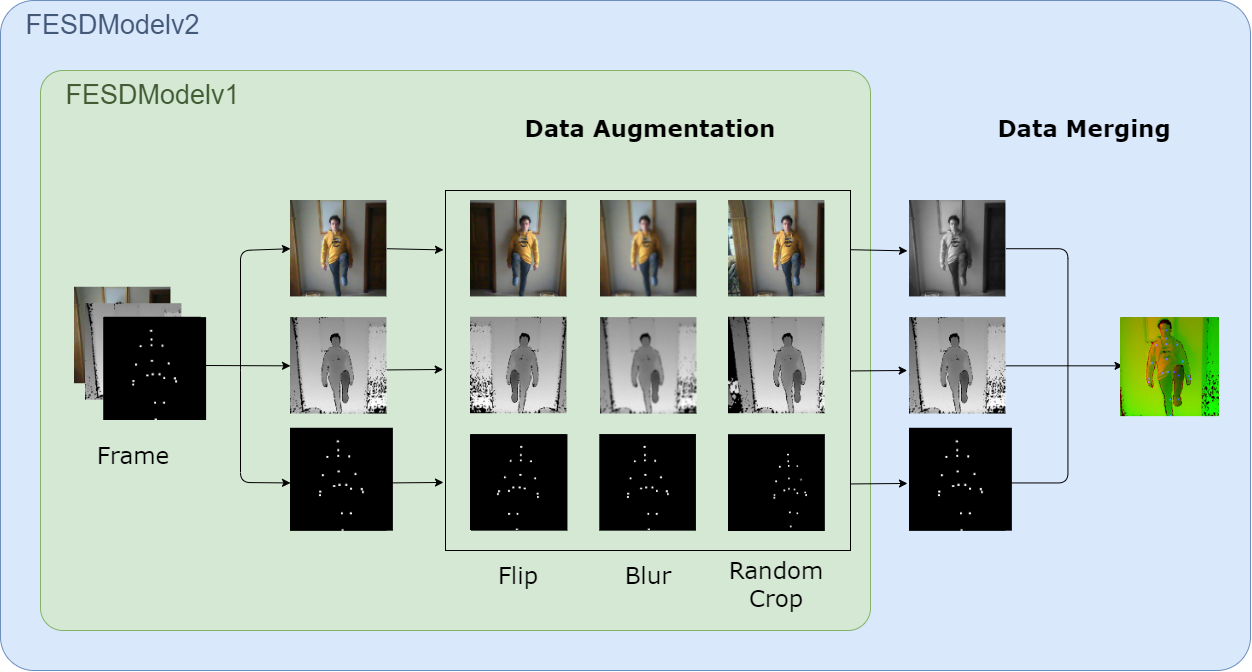
\includegraphics[width=\linewidth]{figures/ProcessingPipeline/DataProcessing.png}
  \caption[Data preparation pipeline for FESDModel]{The three modalities are separately randomly flipped, Blurred, and Cropped. For FESDModelv1 the separate modalities are passed into the network. For FESDModelv2, the RGB image is transformed into a greyscale image and all three modalities are merged into a single RGB image.}
  \label{fig:data_preparation_pipeline}
\end{figure}

The joints are stored within a JSON file containing the coordinates of each joint in 2D and 3D. To process the 2D joint data is drawn on an image that has the same dimensions as the RGB and Depth image for FESDModelv2. For FESDModelv1 the position of each joint relative to the waist joint is passed into the network.

\subsection{Data augmentation}

Four different augmentations are applied to the data to generalise the data. The first augmentation is flipping the data. The RGB image, the depth image, and the joint image are flipped horizontally. Furthermore, the ground truth data is flipped, as labels refer to the left or right side of the body, which would no longer coincide with the data that is passed into the network.

Additionally, the images are cropped at random while keeping the positions of the joints and a margin around the joints visible. This ensures that the model is robust to different positions of the user in the image. 

Finally, Gaussian noise is applied to the RGB image and the depth image. This further improves the robustness of irregular data.

The augmentations can be seen in figure \ref{fig:data_preparation_pipeline} where they are applied to a sample frame from the dataset.

\subsection{Data balancing}

In the ordinary case, HPE is not meant to produce faulty results. In the selected exercises it is aimed to produce faulty results. However, this does still not produce a balanced dataset. In section \ref{sec:dataset}, the statistics of the dataset are shown. Most notably for the problem set \textit{Half} and \textit{Full}, in figures \ref{fig:hb_pie} and \ref{fig:fb_pie}, where the error label \textit{No Error} is overrepresented it can be seen that the dataset is imbalanced.

To balance the dataset, frames are sampled using a Weighted Random Sampler for each batch of the training. The weights for the samples are calculated based on the occurrence of the error labels in the dataset. While only considering the whole body as a single object, the calculation of the weights is simple. For each frame, the error label is counted and the inverse of the count is used as the weight for the frame. This ensures that the model is not biased toward any particular error label by oversampling the frames which contain an error.

However, for the other problem sets the calculation of the weights is more complex. In the other problem sets each frame contains an error for each area, e.g. when considering the Half-Body problem, the upper and lower body 2 errors. To successfully balance the dataset for each area four weights would need to be created and balanced, i.e. the upper and lower body have an error the upper body is faulty and the lower body is not, etc. This would oversample some frames while undersampling others. In the other problem sets this is far more visible. Therefore, it was decided to consider the sum of erroneous joints per frame as a balancing factor. This means that frames that have the same number of erroneous areas are weighed the same.
